\section{Diffusion on Function Spaces}

\begin{frame}{Continuous noising process}
    \begin{figure}
        \centering
        % \vspace{-0.45em}
        \includegraphics[width=.85\textwidth,trim={.1em .2em 0 0},clip]{images/geomndp/1d/noising_rbf.pdf}
        % \centering
        % \includegraphics[width=.85\textwidth,trim={0 0 0 .2em},clip]{images/geomndp/1d/noising_white.pdf}
        \vspace{-0.2em}
    \end{figure}

% We assume we are given a data process $(\fwd_0(x))_{x \in \X}$.
% Given any $\x=(x^1, \dots, x^n) \in \X^n$, we consider the following
 We construct the forward \textbf{noising process} $(\fwd_t(\x))_{t \geq 0} \triangleq (\bfY_t(x^1),\dots,\bfY_t(x^n))_{t \geq 0}$ defined by the multivariate SDE (multivariate Ornstein-Uhlenbeck process)
%
\begin{equation}\label{eq:forward_SDE_sp}
  \textstyle \rmd \fwd_t(\x) = \hlblue{\tfrac{1}{2} \left\{m(\x) -\fwd_t(x) \right\} \beta_t} \rmd t + \hlred{\beta_t^{1/2} \mathrm{K}(\x,\x)^{1/2}}  \rmd \bfB_t,%\quad \fwd_0(\x) = f_0(\x), \ f_0 \sim p_0 ,
\end{equation}
where $\mathrm{K}(\x,\x)_{i,j} = k(x^i, x^j)$ 
% with $k:\rmT^* \X \times \rmT^* \X \rightarrow \R$ a kernel 
with $k:\X \times \X \rightarrow \R$ a kernel 
and $m: \X \rightarrow \Y$.

% The process $(\fwd_t(x))_{t \geq 0}$ is a multivariate Ornstein--Uhlenbeck process---with drift $b(t, \x, \fwd_t(\x)) = m(\x) -\fwd_t(\x)$ and diffusion coefficient $\sigma(t, \x, \fwd_t(\x)) = \mathrm{K}(\x,\x)$---which converges with geometric rate to $\mathrm{N}(m(\x), \mathrm{K}(\x,\x))$.
% Using \cite{phillips2022Spectral}, it can be shown that this convergence extends to the \emph{process} $(\fwd_t)_{t \geq 0}$ which converges to the Gaussian Process with mean $m$ and kernel $k$, denoted $\fwd_\infty $.
%
\pause
\begin{itemize}
    \item $ \fwd_t(\x) \rightarrow \mathrm{N}(m(\x), \mathrm{K}(\x,\x))$ with geometric rate, for any $\x \in \X^n$.
    \item $ \fwd_t \rightarrow \mathrm{GP}(m, k) \triangleq \fwd_\infty$~\cite{phillips2022Spectral}.
    \pause
    \item $\fwd_t$ interpolates between $\fwd_0$ and $\fwd_\infty$.
    \item $\fwd_t(\x)|\bm{y}_0 = \mathrm{N}(m_t(\x; \bm{y}_0), \mathrm{K}_t(\x,\x; \bm{y}_0))$ for any $\x \in \X^n$.
\end{itemize}
    

\end{frame}

\begin{frame}{Continuous noising process}
\begin{figure}
    \centering
    $k(x, x') = k_\mathrm{rbf}(x, x') = \sigma^2 \exp\left(\frac{\| x - x' \|^2}{2 l^2} \right)$, with $l = 1$.
    \vspace{-0.7em}
    \includegraphics[width=.85\textwidth]{images/geomndp/1d/noising_rbf.pdf}
\end{figure}
\pause
\vspace{-0.5em}
\begin{figure}
    \centering
    $k(x, x') = k_\mathrm{rbf}(x, x')$, with $l = 0.2$.
    \vspace{-0.7em}
    \includegraphics[width=.85\textwidth]{images/geomndp/1d/noising_rbf_small2.pdf}
\end{figure}
\pause
\vspace{-0.5em}
\begin{figure}
    \centering
    $k(x, x') = \delta_x(x')$ (The tranditional DDPM settings).
    \includegraphics[width=.85\textwidth]{images/geomndp/1d/noising_white.pdf}
\end{figure}
\end{frame}

% \begin{frame}{Denoising process}
%     As before, the \textbf{time-reversal process} $(\bwd_t(x))_{t \geq 0}$ also satisfies an SDE given by
%     \begin{align}\label{eq:backward_SDE}
%         \textstyle 
%         \rmd \bwd_t(\x) &= {\{-\tfrac{1}{2} (m(\x) - \bwd_t(\x)) + \hlyellow{\mathrm{K}(\x,\x) \nabla \log p_{T-t}(\bwd_t(\x))} \} \beta_{T-t}} \rmd t \nonumber \\
%         &\qquad + {\beta_{T-t}^{1/2} \mathrm{K}(\x,\x)^{1/2}} \rmd \bfB_t, 
%       \end{align}
%       with $\bwd_0 \sim \mathrm{GP} (m, k)$.

% \pause
% To simulate the reverse process we learn the (preconditioned) score
% $$
% \v{s}^K_\theta(t, \bwd_t(x), x) \approx \mathrm{K}(x, x) \nabla \log p_{T-t}(\bwd_t(x)),
% $$
% where $\v{s}^K_\theta: \mathbb{R} \times \mathcal{Y}^m \times \mathcal{X}^m \rightarrow \mathrm{T} \mathcal{Y}^m$.
% We accomplish this using the score matching objective
% $$
% \mathcal{L}(\theta) = \mathbb{E}\left[ \lambda(t) \| \v{s}^K_\theta(t, \fwd_t(x), x) + \mathrm{K}^{1/2} \epsilon \|^2_2\right].
% $$
% \end{frame}

% \begin{frame}{Score approximation}
    
%     % As the reverse SDE \eqref{eq:backward_SDE} involves the preconditioned score $\mathrm{K}(x, x) \nabla \log p_t$, we 
%     \begin{itemize} \setbeamertemplate{itemize items}[triangle]
%         \item We directly approximate $\hlyellow{\mathrm{K}(x, x) \nabla \log p_t}$ with a neural network $\hlyellow{(\mathrm{Ks})_\theta: [0, T] \times \X^n \times \Y^n \rightarrow \rmT \Y^n}$, where $\rmT \Y$ is the tangent bundle of $\Y$.
%         The \textbf{conditional score} of the noising process \eqref{eq:forward_SDE_sp} is given by
%         \begin{equation}
%             \textstyle
%                \hlorange{ \nabla_{{\fwd}_t} \log p_{t}({\fwd}_t(x)| \fwd_0(x))
%                 = - \Sigma_{t|0}^{-1} (\fwd_t(x) - m_{t|0})
%                = - \sigma_{t|0}^{-1} \mathrm{K}(\x,\x)^{-1/2} \varepsilon }, 
%             \end{equation}
%            % \end{align}
%            since $\fwd_t = m_{t|0} + \Sigma_{t|0}^{1/2} \varepsilon$ with $\varepsilon \sim \mathrm{N}(0, \Id)$, 
%            % $m_{t|0} = \mathrm{e}^{-\frac{1}{2} B(t)} \fwd_0$ and 
%            and 
%            $\Sigma_{t|0} = \sigma_{t|0}^2 \mathrm{K}$. % with  $\sigma_{t|0} = (1 - \exp\{-\int_{0}^t \beta(s) \mathrm{d} s\})^{1/2}$.
            
%            \pause
%            \item We learn the \textbf{preconditioned score} $\hlyellow{(\mathrm{Ks})_\theta}$ by minimising the following denoising score matching (DSM) loss~\cite{Vincent2010} weighted by $\Lambda(t) = \sigma_{t|0}^2~\mathrm{K}^\top \mathrm{K}$ 
%            \begin{align*}
%                \label{eq:loss}
%                \textstyle
%                \hlorange{ \mathcal{L}(\theta; \Lambda(t))
%                 = \mathbb{E} [\| \mathrm{s}_\theta(t, \fwd_t) - \nabla \log p_{t}({\fwd}_t| \fwd_0)\|_{\Lambda(t)}^2  ]
%                 = \mathbb{E} [ \| \sigma_{t|0}\cdot \hlyellow{(\mathrm{K}s)_\theta(t,\fwd_t)} + \mathrm{K}^{1/2} \varepsilon \|_2^2 ]} , 
%            \end{align*}
%            where $\|x\|^2_\Lambda = x^\top \Lambda x$.
%     \end{itemize}
    
%     % % and with the preconditoned score network $(\mathrm{K}s)_\theta(t, \cdot) \approx \mathrm{K}(x, x) \nabla \log p_t$.
%     % Note that when targeting a unit-variance white noise, then $\mathrm{K} = \Id$ and the loss \eqref{eq:loss} reverts to the DSM loss with weighting $\lambda(t)=1/\sigma_{t|0}^2$~\cite{song2020score}.

% \end{frame}


% \section{Invariant stochastic processes}
\section{Encoding Invariances}

\begin{frame}{Prior and Conditional Symmetries}
    \vspace{-2.5mm} 
    \begin{figure}[t]
    \centering
    \begin{subfigure}[b]{0.45\textwidth}
    \centering
    \includegraphics[width=1.\linewidth,trim={0 0 0 0},clip]{images/geomndp/1d/prior_ndp_shift.pdf}
    \end{subfigure}%
    \hspace{0.3cm}
    \begin{subfigure}[b]{0.45\textwidth}
    \centering
    \includegraphics[width=1.\linewidth,trim={0 0 0 0},clip]{images/geomndp/2d/prior_ndp_rot.pdf}
    \vspace{-.75em}
    \end{subfigure}
    \end{figure}
    \vspace{-6mm} 
    \begin{figure}[t]
    \centering
    \begin{subfigure}[b]{0.45\textwidth}
    \centering
    \includegraphics[width=1.\linewidth,trim={0 0 0 0},clip]{images/geomndp/1d/conditional_ndp_shift.pdf}
    \end{subfigure}%
    \hspace{0.3cm}
    \begin{subfigure}[b]{0.45\textwidth}
    \centering
    \includegraphics[width=1.\linewidth,trim={0 0 0 0},clip]{images/geomndp/2d/conditional_ndp_rot.pdf}
    \vspace{-.75em}
    \end{subfigure}
    \end{figure}
    
\end{frame}


% \begin{frame}{Invariant stochatic processes}

%     \begin{figure}[t]
%         % \begin{wrapfigure}[20]{r}{.5\linewidth}
%             % \vspace{-.5em}
%             \centering
%              \begin{subfigure}[t]{0.45\textwidth}
%              \centering
%               $G = T(1)$
%               \includegraphics[width=1.\linewidth,trim={0 0 0 0},clip]{images/geomndp/1d/prior_ndp_shift.pdf}
%              \end{subfigure}
%              \begin{subfigure}[t]{0.45\textwidth}
%              \centering
%               $G = O(2)$
%             \includegraphics[width=1.\linewidth,trim={0 0 0 0},clip]{images/geomndp/2d/prior_ndp_rot.pdf}
%             % \vspace{4em}
%             \end{subfigure}
%             \label{fig:prior_model}
%         \end{figure}
 

%     \begin{itemize}
%         \item \textbf{Invariance} A model is G-invariant if it assigns equal probability to $f$ and $g \cdot f$: $p(f) = p(g \cdot f)$.
%         \item \emph{Note: very informal: there is no pdf of a process $f$}.
%     \end{itemize}
% \end{frame}


\begin{frame}{Invariant neural diffusion processes}
    \vspace{3mm}
    \begin{proposition}{Invariant Neural Diffusion Processes}{}
        \label{prop:inv_prior}
    The denoising process on functions as defined above
    % \begin{align}\label{eq:approx_backward_SDE}
    %     \textstyle 
    %     \rmd \bwd_t^\theta(\x) &= \hlblue{\{-\tfrac{1}{2} (m(\x) - \bwd_t(\x)) + \mathbf{s}^K_\theta(T - t, \x, \bwd_t(\x)) \} \beta_{T-t}} \rmd t \nonumber \\
    %     &\quad + \hlred{\beta_{T-t}^{1/2} \mathrm{K}(\x,\x)^{1/2}} \rmd \bfB_t,
    %   \end{align}
    %  the time-reversal SDE \eqref{eq:backward_SDE} where the score is approximated by a score network $\mathbf{s}_\theta: [0, T] \times \X^n \times \Y^n \rightarrow \rmT \Y^n$, 
     and with initial sample given by $p(\bar{\fwd}_0) = \mathrm{GP}(m, k)$ is G-invariant if
     \begin{enumerate}
        \item $m$ and $k$ are both $G$-equivariant (i.e. G-invariant Gaussian process), i.e.
        $$
        m(g \cdot x) = \rho(g) m(x)\quad\text{and}\quad k(g \cdot x, g \cdot x') = \rho(g)k(x,x')\rho(g)^\top,
        $$
        \item the score network is $G$-equivariant vector field, i.e.
        $$
        \mathbf{s}_\theta(t, g\cdot \x, \rho(g) \y) = \rho(g) \mathbf{s}_\theta(t, \x, \y),
        $$
        for all $\x \in \X, g \in G.$
     \end{enumerate}
    \end{proposition}

\end{frame}

% \begin{frame}{Invariant Gaussian processes}
    
%     \begin{proposition}{Invariant (stationary) Gaussian process \cite{holderrieth2021equivariant}.}{}
%         \label{prop:inv_gp}
%         We have that a Gaussian process $\mathrm{GP}(m, k)$ is $G$-invariant if and only if its mean $m$ and covariance $k$ are $G$-equivariant---that is, for all $\x,\x' \in \X, g \in G$
%     \begin{align}
%     m(g \cdot \x) = \rho(g) m(\x) \ \ \text{and} \ \ k(g \cdot \x, g \cdot \x') = \rho(g) k(\x, \x') \rho(g)^\top.
%     \end{align}
%     \end{proposition}
    
    % $\mathrm{E}(d)$-equivariant kernels include
    % \vspace{-0.5em}
    % \begin{itemize}
    %     \item Diagonal kernels $k = k_0 \Id$ with $k_0$ invariant~\cite{holderrieth2021equivariant}.
    %     \item $k_\mathrm{curl} = k_0 A$ with $A(x, x') = \mathrm{I} - \frac{(x - x')(x - x')^\top}{l^2}$ ~\cite{macedo2010learning}.
    %     \item $k_\mathrm{div} = k_0 B$ with $ B(x, x') =\frac{(x - x')(x - x')^\top}{l^2} + \left( n -1 - \frac{\|x - x' \|^2}{l^2} \right) \mathrm{I}$. %~\cite{macedo2010learning}
    % \end{itemize}

%     A kernel $k: \rset^d \times \rset^d \rightarrow \rset^{d\times d}$ is equivariant if it satisfies the following constraints:
% %
% (a) $k$ is \emph{stationnary}, that is if for all $x, x' \in \R^n$ 

% \begin{align}
%    k(x, x') = k(x - x') \triangleq \tilde{k}(x - x')
% \end{align}
% and if (b) it satisfies the \emph{angular constraint} for any $h \in H$
% \begin{align}
%    k(h x, h x') = \rho(h) k(x, x') \rho(h)^\top.
% \end{align}

% A trivial example of such an equivariant kernel is the diagonal kernel $k(x,x') = k_0(x, x') \mathrm{I}$ \citep{holderrieth2021equivariant}, with $k_0$ stationnary.
% This kernel can be understood has having $d$ independent Gaussian process uni-dimensional output, that is, there is no inter-dimensional correlation.

% Less trivial examples, are the $\mathrm{E}(d)$ equivariant kernels proposed in \citet{macedo2010learning}.
% Namely curl-free and divergence-free kernels, allowing for instance to model electric or magnetic fields.
% Formally we have
% $k_\mathrm{curl} = k_0 A$ and $k_\mathrm{div} = k_0 B$
% with $k_0$ stationary, e.g.\ squared exponential kernel $k_0(x, x') = \sigma^2 \exp\left(\frac{\| x - x' \|^2}{2 l^2} \right)$, and $A$ and $B$ given by
% %
% \begin{align}
%     A(x, x') = \mathrm{I} - \frac{(x - x')(x - x')^\top}{l^2}
% \end{align}
% \begin{align}
%     B(x, x') = \frac{(x - x')(x - x')^\top}{l^2} + \left( n -1 - \frac{\|x - x' \|^2}{l^2} \right) \mathrm{I}.
% \end{align}

% \end{frame}


% \begin{frame}{$\mathrm{E}(d)$-invariant Gaussian processes}
    
%     \begin{center}
%         \includegraphics[width=.72\textwidth]{images/geomndp/2d/e2_equiv_kernels.png}
%     \end{center}

%     \begin{itemize}
%     \item $\mathrm{E}(d)$-equivariant means $m: \rset^d \rightarrow \rset^d$ are constant functions.
%     \pause
%     \item $\mathrm{E}(d)$-equivariant kernels $k: \rset^d \times \rset^d \rightarrow \rset^{d\times d}$ include
%     % \vspace{-0.5em}
%     \begin{itemize} \setbeamertemplate{itemize items}[triangle]
%         \item Diagonal kernels $k = k_0 \Id$ with $k_0$ invariant~\cite{holderrieth2021equivariant}.
%         \item $k_\mathrm{curl} = k_0 A$ with $A(x, x') = \Id - \frac{(x - x')(x - x')^\top}{l^2}$ ~\cite{macedo2010learning}.
%         \item $k_\mathrm{div} = k_0 B$ with $ B(x, x') =\frac{(x - x')(x - x')^\top}{l^2} + \left( n -1 - \frac{\|x - x' \|^2}{l^2} \right) \Id$. %~\cite{macedo2010learning}
%     \end{itemize}
% \end{itemize}

% \end{frame}




% \begin{frame}{Invariant neural diffusion processes (Cont'd)}
    
%     \begin{figure}[t]
%     \vspace{-0.5em}
%     \centering
%         \includegraphics[width=.95\textwidth]{images/geomndp/2d/steerable_noising.pdf}
%         \vspace{-.5em}
%         \caption{
%             $(g \cdot {\fwd}_t(x))_{x \in \X}$
%             }
%         \label{fig:equiv_noising_model}
%     \end{figure}

% \end{frame}

% \section{Conditional processes}

% \begin{frame}{Equivariant conditional processes}
%     Let $\mathcal{C} = \{(x_n, y_n)\}_{n}$ be a context dataset of input and ouptut pair.
%     A conditional distribution $p(f\mid \mathcal{C})$ is equivariant to the action $g$
%     $$
%     p(f\mid \mathcal{C}) = p(g^{-1} \cdot f\mid g \cdot \mathcal{C}).
%     $$
%     \pause
%     % A stochastic process with distribution $\mu$ given a context $\mathcal{C}$
%     % is said to be conditionally $G-$equivariant if the conditional satisfies
%     % $\hlorange{\mu(\mathsf{A} | g \cdot \mathcal{C}) = \mu(g \cdot \mathsf{A}
%     % |\mathcal{C})}$, or equivalently  $\hlorange{\mu(g^{-1} \cdot \mathsf{A} | g
%     % \cdot \mathcal{C}) = \mu(\mathsf{A} |\mathcal{C})}$, for any $g \in G$ and
%     % $\mathsf{A} \in \mathrm{C}(\mathcal{X},\mathcal{Y})$ measurable.
%     \vspace{-1em}
%     \begin{figure}[t]
%         % \begin{wrapfigure}[20]{r}{.5\linewidth}
%             \vspace{-1em}
%             \centering
%              \begin{subfigure}[b]{0.49\textwidth}
%              \centering
%              \vspace{0.em}
%               \includegraphics[width=1.\linewidth,trim={0 0 0 0},clip]{images/geomndp/1d/conditional_ndp_shift.pdf}
%             % \includegraphics[width=.48\linewidth,trim={0 0 0 0},clip]{../figs/1d_conditional.png}
%             % \includegraphics[width=.48\linewidth,trim={0 0 0 0},clip]{../figs/1d_conditional_shift.png}
%              \end{subfigure}
%              \begin{subfigure}[b]{0.49\textwidth}
%              \centering
%              \vspace{0.em}
%             \includegraphics[width=1.\linewidth,trim={0 0 0 0},clip]{images/geomndp/2d/conditional_ndp_rot.pdf}
%             % \includegraphics[width=.48\linewidth,trim={40em 0 0 0},clip]{../figs/conditional_ndp_rot.png}
%             %  \includegraphics[width=.48\linewidth,trim={4em 0 36em 0},clip]{../figs/conditional_ndp_rot.png}
%             \vspace{-.75em}
%             % \vfill
%             \end{subfigure}
%             \vspace{-0.5em}
%             \caption{\footnotesize
%             Samples conditioned on context set $\mathcal{C}$ (\textcolor{C3}{in red}) for scalar (\emph{Left}) and 2D vector (\emph{Right}) fields.
%             Same model is then conditioned on transformed context $g \cdot \mathcal{C}$. %, with group element $g$ being a translation of length $2$ (\emph{Left}) or a $90^{\circ}$ rotation (\emph{Right}).
%             }
%             \label{fig:posterior_model}
%         \end{figure}
 
% \end{frame}

% \begin{frame}{Equivariant conditional processes}
%     \begin{proposition}{Equivariant conditional process.}{}
%         \label{prop:equiv_posterior}
%         Assume a stochastic process $f \sim \mu$ is  $G-$invariant. Then the conditional process $f|\mathcal{C}$ given a set of observations $\mathcal{C}$ is $G$-equivariant. % in the sense $$g\cdot(f|\c{C}) \overset{d}{=} f|(g \cdot \c{C})$$
%     \end{proposition}
% \end{frame}

\section{Conditional Process}

\begin{frame}{Conditional sampling in diffusion models}
\textbf{Goal:} Sample from $y \sim p(\cdot \mid \mathcal{C})$ given a condition $\mathcal{C}$.\\
\pause
\begin{figure}
\centering
\includegraphics[width=\linewidth]{images/conditional_dalle.png}
\caption{$p(image \mid text)$}
\end{figure}
Often the condition is a property (e.g., caption).
\end{frame}

\begin{frame}{Conditional sampling in diffusion models for functions}
% \textbf{Goal:} Sample from $y \sim p(\cdot \mid \mathcal{C})$ given a condition $\mathcal{C}$.\\

Condition is a subspace of the state space: $y = (y^{(1)}, \ldots, y^{(m)})$ and $\mathcal{C} = (y^{(m+1)},\ldots, y^{(n)})$.
\pause
\begin{figure}
\centering
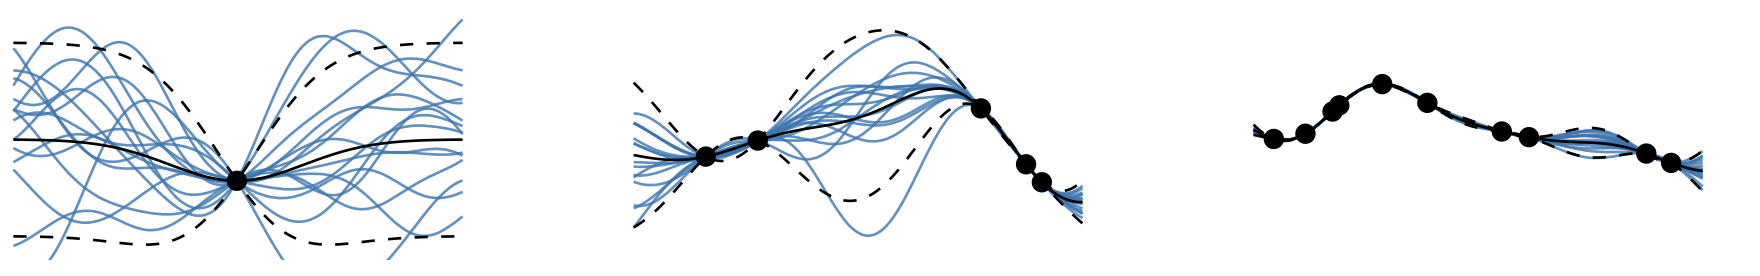
\includegraphics[width=\linewidth]{images/conditioning_gp.png}
% \includegraphics[width=\linewidth,trim={5cm 0 5cm 0},clip]{images/example_2d/conditional.pdf}
\caption{Conditional samples $p(y^*\mid \mathcal{C})$.}
\end{figure}
\end{frame}


\begin{frame}{Conditional sampling in diffusion models}
In the reverse process we need to follow the \textbf{Conditional Score}
$$
\nabla \log p_t(\fwd_t) \implies \nabla \log p_t(\fwd_t \mid \mathcal{C})
$$
\pause
\begin{enumerate}
    \item Amortisation / Classifier-free ~\cite{ramesh2022Hierarchical}
    \item Classifier-guidance~\cite{dhariwal2021diffusion}
    \item Replacement methods {RePaint}~\cite{lugmayr2022RePaint}
    \item Reconstruction guidance~\cite{finzi2023user}
    \item SMC-based~\cite{trippe2022Diffusion}
\end{enumerate}
\end{frame}


\begin{frame}{Langevin Dynamics based Conditional Sampling}
Focussing on the function setting, the context $\mathcal{C} = \fwd_0^\mathcal{C}$
\begin{align*}
\nabla_{\fwd_t} \log p_t(\fwd_t \mid \fwd_0^\mathcal{C})
&= \nabla_{\fwd_t} \log p_t(\fwd_t, \fwd_0^\mathcal{C}) - \nabla_{\fwd_t} \log p_t(\fwd_0^\mathcal{C})\\
&= \nabla_{\fwd_t} \log p_t(\fwd_t, \fwd_0^\mathcal{C})
\end{align*}
\pause
\begin{center}
\begin{minipage}[c]{0.8\linewidth}
\begin{itemize}
    \item[\textcolor{C0}{Predictor}] Use standard EM reverse process with score $s_\theta^K(t, x, [\fwd_t, \fwd_0^\mathcal{C}])$.
    \item[\textcolor{C3}{Corrector}] Correct discretisation errors using Langevin dynamics
\end{itemize}
\end{minipage}
\end{center}
\pause
\vspace{-5em}
\begin{figure}
    \centering
    \begin{center}
    \resizebox{.7\linewidth}{!}{
    \begin{tikzpicture}
    \Large
        \draw [stealth-, line width = .05cm] (0,0) .. controls  (2,-4) and (3.,2) .. (6,0);
        \draw [-stealth, line width = .05cm, C0, dashed] (0,0) -- (1.3,-2.3);
        \draw [-stealth, line width = .05cm, C3, dashed] (1.3,-2.3) -- (1.3,-1.9);
        \draw [-stealth, line width = .05cm, C3, dashed] (1.3,-1.9) -- (1.3,-1.7);
        \draw [-stealth, line width = .05cm, C3, dashed] (1.3,-1.7) -- (1.3,-1.4);
        \draw [-stealth, line width = .05cm, C0, dashed] (1.3,-1.45) -- (2.8,-1.35);
        \draw [-stealth, line width = .05cm, C3, dashed] (2.8,-1.35) -- (2.4, -0.9);
    %   \draw [-stealth, line width = .05cm, blue, dashed] (0,0) -- (1.3,-2.3);
    %   \draw [-stealth, line width = .05cm, red, dashed] (1.3,-2.3) -- (1.3,-1.2);
    %   \draw [-stealth, line width = .05cm, blue, dashed] (1.3,-1.2) -- (2.8,-0.7);
    %   \draw [-stealth, line width = .05cm, red, dashed] (2.8,-0.7) -- (2.6, -0.5);
        \node [below=0.2cm] at (6,0) {\footnotesize $p_0$};
        \node [left=0.0cm] at (0,0) {\footnotesize $p(\bwd_0) = p_T$};
        \node [left=0.2cm] at (1.3,-2.1) {\footnotesize $p(\bwd_\gamma^0)$};
        \node [right=0.1cm] at (1.3,-2.) {\footnotesize $p(\bwd_\gamma^1)$};
        \node [right=0.1cm] at (1.3,-1.65) {\footnotesize $\cdots$};
    %   \node [below right=0.1cm] at (1.3,-1.2) {$\mathcal{L}(\fwd_\gamma^1)$};
    %   \node [above=0.05cm] at (1.3,-1.2) {$\mathcal{L}(\fwd_\gamma^3)$};
        \node [above=0.05cm] at (1.3,-1.35) {\footnotesize $p_{\gamma}$};
    %   \node [right=0.2cm] at (2.8,-0.7) {$\mathcal{L}(\fwd_{2\gamma}^0)$};
        %   \node [above left=0.1cm] at (2.6, -0.5) {$\mathcal{L}(\fwd_{2\gamma}^1)$};
        \node [below right=0.1cm] at (2.8,-0.8) {\footnotesize $p(\bwd_{2\gamma}^0)$};
        \node [right=0.1cm] at (2.6, -0.7) {\footnotesize $p(\bwd_{2\gamma}^1)$};
        \node [above left=0.05cm] at (2.6, -0.9) {\footnotesize $p_{2\gamma}$};
    \end{tikzpicture}
    }
    \end{center}
    \vspace{-3.5em}
    \end{figure}
\end{frame}


% \begin{frame}{Conditional neural diffusion processes: Predictor}

%     \begin{itemize} \setbeamertemplate{itemize items}[triangle]
%         \item \textbf{Aim}: Sample $y^* \sim p(\cdot|x^*, \mathcal{C})$ given a set of observations context $\mathcal{C} = \{(x^c, y^c)\}_{c \in C}$.
%         \item \textbf{Predictor}: Single-step backward: $\fwd_{t - \gamma}^*, \fwd_{t - \gamma}^c \gets \fwd_{t}^*, \fwd_{t}^c$

%         \begin{itemize}
%         % \item $\color{algcol}{\v{y}^c_t \sim p_{t, \v{x}^c}(\v{y}^c_t | \v{y}^c_0)}$
%         \item \textbf{Noise context}: $\color{algcol}{\bfY_{t}^c|\bfY_{0}^c \sim p_{t|0}}$
%         \item \textbf{Denoise joint}: 
%         with $\x \triangleq [x^*, x^c]$\\
%         $\sbr{\text{\_}, \tilde{\fwd}_{t-\gamma}^*} = \sbr{\textcolor{algcol}{\fwd^c_t}, {\fwd}_t^*} + \gamma \left\{ -\frac{1}{2} \left( m({\x}) - \sbr{\textcolor{algcol}{\fwd^c_t}, {\fwd}_t^*} \right) + \mathbf{Ks}_\theta(t, {\x}, \sbr{\textcolor{algcol}{\fwd^c_t}, \tilde{\fwd}_t^*}) \right\} + \sqrt{\gamma} \mathrm{K}({\x}, {\x})^{1/2} Z$
%         \end{itemize}
%     \end{itemize}
%     \pause
%     \begin{figure}
%         \centering
%         \includegraphics[width=0.6\textwidth,trim={0 73em 88em 0},clip]{images/geomndp/noised_replacement_sampling.pdf}
%         % \caption{Ablation of number of corrector steps for conditional sampling.}
%         % \label{fig:app:conditional-ablation}
%     \end{figure}

%     \begin{itemize} \setbeamertemplate{itemize items}[triangle]
%         \item \textbf{Exact} as $\gamma \rightarrow 0$, or can correct with SMC~\cite{trippe2022Diffusion}.
%         \item \textbf{Problem}: In practice even with tiny $\gamma$ tend to dismiss context $\mathcal{C}$ !
%     \end{itemize}

 
% \end{frame}


% \begin{frame}{Conditional neural diffusion processes: Corrector}
%     \vspace{2em}
%     \begin{itemize} \setbeamertemplate{itemize items}[triangle]
%         % \item \textbf{Aim}: Sample $y^* \sim p(\cdot|x^*, \mathcal{C})$ given observations $\mathcal{C} = \{(x^c, y^c)\}_{c \in C}$.
%         \item \textbf{Corrector}: (Multi-steps to) Target $p_t(\y_{t}^*|\y_{t}^c)$
%         \begin{itemize}
%         \item  \textsc{RePaint}~\cite{lugmayr2022RePaint}: denoise and re-noise $[\fwd_t^*, \fwd_t^c]$ to increase correlation.
%         \item Note that $\nabla_{y_t^*} \log p(y_t^*|y_t^c) = \nabla_{y_t^*} \log p(y_t^*, y_t^c) - \nabla_{y_t^*} \log p(y_t^c) = \nabla_{y_t^*} \log p(y_t^*, y_t^c)$
%         \item Langevin dynamics $\rmd \fwd_s^* = \tfrac{1}{2} \mathrm{K} \nabla_{\fwd_s^*} \log p_{T-t}(\fwd_s^*, \fwd_s^c) \rmd s +  \sqrt{\mathrm{K}} \rmd \bfB_s$
%     \end{itemize} 
%     \end{itemize}

%     \begin{figure}
%         \vspace{-3.5em}
%         \centering
%         \begin{center}
%         \resizebox{.55\linewidth}{!}{
%         \begin{tikzpicture}
%         \Large
%           \draw [stealth-, line width = .05cm] (0,0) .. controls  (2,-4) and (3.,2) .. (6,0);
%           \draw [-stealth, line width = .05cm, C0, dashed] (0,0) -- (1.3,-2.3);
%           \draw [-stealth, line width = .05cm, C3, dashed] (1.3,-2.3) -- (1.3,-1.9);
%           \draw [-stealth, line width = .05cm, C3, dashed] (1.3,-1.9) -- (1.3,-1.7);
%           \draw [-stealth, line width = .05cm, C3, dashed] (1.3,-1.7) -- (1.3,-1.4);
%           \draw [-stealth, line width = .05cm, C0, dashed] (1.3,-1.45) -- (2.8,-1.35);
%           \draw [-stealth, line width = .05cm, C3, dashed] (2.8,-1.35) -- (2.4, -0.9);
%         %   \draw [-stealth, line width = .05cm, blue, dashed] (0,0) -- (1.3,-2.3);
%         %   \draw [-stealth, line width = .05cm, red, dashed] (1.3,-2.3) -- (1.3,-1.2);
%         %   \draw [-stealth, line width = .05cm, blue, dashed] (1.3,-1.2) -- (2.8,-0.7);
%         %   \draw [-stealth, line width = .05cm, red, dashed] (2.8,-0.7) -- (2.6, -0.5);
%           \node [below=0.2cm] at (6,0) {$p_0$};
%           \node [left=0.0cm] at (0,0) {$\mathcal{L}(\bwd_0) = p_T$};
%           \node [left=0.2cm] at (1.3,-2.1) {$\mathcal{L}(\bwd_\gamma^0)$};
%           \node [right=0.1cm] at (1.3,-2.) {$\mathcal{L}(\bwd_\gamma^1)$};
%           \node [right=0.1cm] at (1.3,-1.65) {$\cdots$};
%         %   \node [below right=0.1cm] at (1.3,-1.2) {$\mathcal{L}(\fwd_\gamma^1)$};
%         %   \node [above=0.05cm] at (1.3,-1.2) {$\mathcal{L}(\fwd_\gamma^3)$};
%           \node [above=0.05cm] at (1.3,-1.35) {$p_{\gamma}$};
%         %   \node [right=0.2cm] at (2.8,-0.7) {$\mathcal{L}(\fwd_{2\gamma}^0)$};
%             %   \node [above left=0.1cm] at (2.6, -0.5) {$\mathcal{L}(\fwd_{2\gamma}^1)$};
%           \node [below right=0.1cm] at (2.8,-0.8) {$\mathcal{L}(\bwd_{2\gamma}^0)$};
%           \node [right=0.1cm] at (2.6, -0.7) {$\mathcal{L}(\bwd_{2\gamma}^1)$};
%           \node [above left=0.05cm] at (2.6, -0.9) {$p_{2\gamma}$};
%         \end{tikzpicture}
%         }
%         \end{center}
%         \vspace{-3.5em}
%         \caption{
%         Illustration of Langevin corrected conditional sampling.
%         The black line represents the noising process dynamics $(p_t)_{t \in \ccint{0,T}}$.
%         The \textcolor{C0}{time reversal (i.e.\ predictor)} step, is combined with a \textcolor{C3}{Langevin corrector} step projecting back onto the dynamics.
%           % The black line corresponds to the dynamics of the noising process 
%           % $(p_t)_{t \in \ccint{0,T}}$.
%           % The \textcolor{C0}{blue dashed lines} correspond to the predictor step (going backward in time) and the \textcolor{C3}{red dashed lines} correspond to
%           % the corrector step (projecting back onto the forward dynamics).
%         }
%         \label{fig:predictor_corrector}
%         \end{figure}
%     % \end{wrapfigure}
 
% \end{frame}


% \begin{frame}{Conditional neural diffusion processses: Langevin corrector}
%     % \begin{figure}
%     %     \centering
%     %     \includegraphics[width=0.5\textwidth]{images/geomndp/compare_noising_schemes.pdf}
%     %     \caption{Ablation noising schemes for conditional sampling.}
%     %     \label{fig:app:conditional-ablation}
%     % \end{figure}
%     \begin{figure}
%         \centering
%         % \includegraphics[width=\textwidth]{images/geomndp/1d/conditional_ablation.pdf}
%         \includegraphics[width=0.6\textwidth]{images/geomndp/1d/conditional_ablation.png}
%         \caption{Ablation of number of corrector steps for conditional sampling.}
%         % \label{fig:app:conditional-ablation}
%     \end{figure}
% \end{frame}


% \begin{frame}{Predictive log-likelihood}
%     %
%     \begin{center}
%         \includegraphics[width=0.9\textwidth]{images/sde.png}
%     \end{center}
%     %
%     We can derive a deterministic process which has the same marginal density as the noising SDE \eqref{eq:forward_SDE_sp}, which  given by the following ODE
%     % is given by the following Ordinary Differential Equation (ODE)---referred as the probability flow ODE~\cite{song2020score}
%     %
%     \begin{align*}%\label{eq:backward_SDE}
%         \textstyle 
%         \rmd \tilde{\fwd}_t(\x) &= \hlblue{\{\tfrac{1}{2} (m(\x) - \bwd_t(\x)) - \tfrac{1}{2} \mathrm{K}(\x,\x) \nabla \log p_{T-t}(\bwd_t(\x)) \} \beta_{t}} \rmd t
%         \triangleq \hlblue{f_{\mathrm{ODE}}(t, x, \fwd_t(\x))} \rmd t 
%       \end{align*}
%     %   with $\bwd_0 \sim \mathrm{GP} (m, k)$ and $p_t$ the density of $\mathbf{Y}_t(x)$ w.r.t.~the Lebesgue measure.
%     %
%     \begin{align} \label{eq:probability_flow_ode}
%     \rmd 
%     \begin{pmatrix}
%         \hspace{2.2em}  \tilde{\fwd}_t(\x)  \\
%         \log p_t(\tilde{\fwd}_t(\x))
%       \end{pmatrix}
%       = 
%       %   \begin{pmatrix}
%       %     \hspace{2em} \tfrac{1}{2}  \left\{ m(\x) - \fwd_t(\x) -  \mathrm{K}(\x,\x) \nabla \log p_t( \fwd_t(\x)) \right\} \beta_t \\
%       %      - \tfrac{1}{2}  \dive \left\{ m(\x) - \fwd_t(\x) -  \mathrm{K}(\x,\x) \nabla \log p_t( \fwd_t(\x)) \right\} \beta_t 
%       %   \end{pmatrix}
%       \hlblue{
%       \begin{pmatrix}
%         \hspace{2em} f_{\mathrm{ODE}}(t, x, \fwd_t(\x)) \\
%          - \tfrac{1}{2}  \dive~ f_{\mathrm{ODE}}(t, x, \fwd_t(\x)) 
%       \end{pmatrix}
%       }
%       \rmd t.
%     \end{align}
        
%     \end{frame}


\section{Experimental results}

\begin{frame}{1D regression: Datasets}
    \begin{center}
        % \includegraphics[width=.85\textwidth]{images/geomndp/1d/plot_regression1d_body.pdf}
        \includegraphics[trim={0 0.8em 0 0},clip, width=.75\textwidth]{images/geomndp/1d/plot_regression1d_appendix.pdf}
    \end{center}
    
\end{frame}

% \begin{frame}{1D regression: Predictive log-likelihood}
% %
% \begin{center}
%     \includegraphics[width=0.9\textwidth]{images/sde.png}
% \end{center}
% %
% We can derive a deterministic process which has the same marginal density as the noising SDE \eqref{eq:forward_SDE_sp}, which  given by the following ODE
% % is given by the following Ordinary Differential Equation (ODE)---referred as the probability flow ODE~\cite{song2020score}
% %
% \begin{align*}%\label{eq:backward_SDE}
%     \textstyle 
%     \rmd \tilde{\fwd}_t(\x) &= \hlblue{\{\tfrac{1}{2} (m(\x) - \bwd_t(\x)) - \tfrac{1}{2} \mathrm{K}(\x,\x) \nabla \log p_{T-t}(\bwd_t(\x)) \} \beta_{t}} \rmd t
%     \triangleq \hlblue{f_{\mathrm{ODE}}(t, x, \fwd_t(\x))} \rmd t 
%   \end{align*}
% %   with $\bwd_0 \sim \mathrm{GP} (m, k)$ and $p_t$ the density of $\mathbf{Y}_t(x)$ w.r.t.~the Lebesgue measure.
% %
% \begin{align} \label{eq:probability_flow_ode}
% \rmd 
% \begin{pmatrix}
%     \hspace{2.2em}  \tilde{\fwd}_t(\x)  \\
%     \log p_t(\tilde{\fwd}_t(\x))
%   \end{pmatrix}
%   = 
%   %   \begin{pmatrix}
%   %     \hspace{2em} \tfrac{1}{2}  \left\{ m(\x) - \fwd_t(\x) -  \mathrm{K}(\x,\x) \nabla \log p_t( \fwd_t(\x)) \right\} \beta_t \\
%   %      - \tfrac{1}{2}  \dive \left\{ m(\x) - \fwd_t(\x) -  \mathrm{K}(\x,\x) \nabla \log p_t( \fwd_t(\x)) \right\} \beta_t 
%   %   \end{pmatrix}
%   \hlblue{
%   \begin{pmatrix}
%     \hspace{2em} f_{\mathrm{ODE}}(t, x, \fwd_t(\x)) \\
%      - \tfrac{1}{2}  \dive~ f_{\mathrm{ODE}}(t, x, \fwd_t(\x)) 
%   \end{pmatrix}
%   }
%   \rmd t.
% \end{align}
    
% \end{frame}

\begin{frame}{1D regression: Predictive log-likelihood (Cont'd)}
    % \begin{center}

        \begin{table}[b]
            \small
            \centering
            \caption{
                Mean test log-likelihood (TLL) ($\uparrow$) $\pm$ 1 standard error estimated over 4096 test samples are reported.
                % Statistically significant best non-GP model is in \textbf{bold}.
                % `*' stands for a TLL below $-10$.
                NP baselines from \cite{bruinsma2020Gaussian}.
                \label{tab:1d_regression}
                }
        \setlength{\tabcolsep}{2.pt}
        % \begin{tabular}{llccccc}
        \begin{tabular}{llrrrrr}
        \toprule
         & & \multicolumn{1}{c}{\scshape SE} & \multicolumn{1}{c}{\scshape Mat\'ern$(\tfrac52)$} & \multicolumn{1}{c}{\scshape Weakly Per.} & \multicolumn{1}{c}{\scshape Sawtooth} & \multicolumn{1}{c}{\scshape Mixture}\\
        
        \midrule
        % \multicolumn{6}{l}{\textsc{Interpolation}} \\[0.5em]
         \parbox[t]{2mm}{\multirow{5}{*}{\rotatebox[origin=c]{90}{\textsc{\scalefont{.85} Interpolat}.}}}
         & \scshape GP (optimum)& $\hphantom{-}0.70 { \pm \scriptstyle 0.00 }$& $\hphantom{-}0.31 { \pm \scriptstyle 0.00 }$& $-0.32 { \pm \scriptstyle 0.00 }$& - & - \\
        % \rowcolor{pearDark!20}
        & \cellcolor{pearDark!20}\scshape $\mathrm{T}(1)-$\method & \cellcolor{pearDark!20} $\hphantom{-}\mathbf{0.72} { \pm \scriptstyle 0.03 }$& \cellcolor{pearDark!20} $\hphantom{-}\mathbf{0.32} { \pm \scriptstyle 0.03 }$& \cellcolor{pearDark!20} $\mathbf{-0.38} { \pm \scriptstyle 0.03 }$& \cellcolor{pearDark!20} $\hphantom{-}\mathbf{3.39} { \pm \scriptstyle 0.04 }$& \cellcolor{pearDark!20} $\hphantom{-}\mathbf{0.64} { \pm \scriptstyle 0.08 }$\\
        % \rowcolor{pearDark!20} 
        & \scshape NDP\textsuperscript{*} &  $\hphantom{-}\mathbf{0.71} { \pm \scriptstyle 0.03 }$&  $\hphantom{-}\mathbf{0.30} { \pm \scriptstyle 0.03 }$&  $\mathbf{-0.37} { \pm \scriptstyle 0.03 }$&  $\hphantom{-}\mathbf{3.39} { \pm \scriptstyle 0.04 }$&  $\hphantom{-}\mathbf{0.64} { \pm \scriptstyle 0.08 }$\\
        & \scshape GNP& $\hphantom{-}\mathbf{0.70} { \pm \scriptstyle 0.01 }$& $\hphantom{-}\mathbf{0.30} { \pm \scriptstyle 0.01 }$& $-0.47 { \pm \scriptstyle 0.01 }$& $\hphantom{-}0.42 { \pm \scriptstyle 0.01 }$& $\hphantom{-}0.10 { \pm \scriptstyle 0.02 }$\\
        & \scshape ConvNP& $-0.46 { \pm \scriptstyle 0.01 }$& $-0.67 { \pm \scriptstyle 0.01 }$& $-1.02 { \pm \scriptstyle 0.01 }$& $\hphantom{-}1.20 { \pm \scriptstyle 0.01 }$& $-0.50 { \pm \scriptstyle 0.02 }$\\
        
        \midrule
        \parbox[t]{2mm}{\multirow{5}{*}{\rotatebox[origin=c]{90}{\textsc  {\scalefont{.85} Generalisat}.}}}
        & \scshape GP (optimum)& $\hphantom{-}0.70 { \pm \scriptstyle 0.00 }$& $\hphantom{-}0.31 { \pm \scriptstyle 0.00 }$& $-0.32 { \pm \scriptstyle 0.00 }$& -& -\\
        & \cellcolor{pearDark!20}\scshape$\mathrm{T}(1)-$\method & \cellcolor{pearDark!20} $\hphantom{-}\mathbf{0.70} { \pm \scriptstyle 0.02 }$& \cellcolor{pearDark!20} $\hphantom{-}\mathbf{0.31} { \pm \scriptstyle 0.02 }$& \cellcolor{pearDark!20} $\mathbf{-0.38} { \pm \scriptstyle 0.03 }$& \cellcolor{pearDark!20} $\hphantom{-}\mathbf{3.39} { \pm \scriptstyle 0.03 }$& \cellcolor{pearDark!20} $\hphantom{-}\mathbf{0.62} { \pm \scriptstyle 0.02 }$\\
        &  \scshape NDP\textsuperscript{*} & *& *& *& *& *\\
        & \scshape GNP& $\hphantom{-}\mathbf{0.69} { \pm \scriptstyle 0.01 }$& $\hphantom{-}\mathbf{0.30} { \pm \scriptstyle 0.01 }$& $-0.47 { \pm \scriptstyle 0.01 }$& $\hphantom{-}0.42 { \pm \scriptstyle 0.01 }$& $\hphantom{-}0.10 { \pm \scriptstyle 0.02 }$\\
        & \scshape ConvNP& $-0.46 { \pm \scriptstyle 0.01 }$& $-0.67 { \pm \scriptstyle 0.01 }$& $-1.02 { \pm \scriptstyle 0.01 }$& $\hphantom{-}1.19 { \pm \scriptstyle 0.01 }$& $-0.53 { \pm \scriptstyle 0.02 }$\\
        \bottomrule
        \end{tabular}
        \end{table}
      
    % \end{center}
    
\end{frame}


% \begin{frame}{1D regression: Kernel ablation}

%     \begin{center}
%         \includegraphics[width=.9\textwidth]{images/geomndp/1d/ablation.png}
%         \captionof{figure}{Ablation study targeting different limiting kernels and score parametrisations.}
%     \end{center}    

% \end{frame}


\begin{frame}{2D invariant Gaussian vector fields}
    \begin{center}
        \includegraphics[width=.72\textwidth]{images/geomndp/2d/e2_equiv_kernels.png}
    \end{center}
    
    \vspace{-1em}
    \begin{table}
        \small
        \centering
        \begin{tabular}{lccc}
            \toprule
            \textsc{Model} & \scshape SE & \scshape Curl-free & \scshape Div-free \\
            \midrule
            \scshape GP & ${0.56_{\pm 0.00}}$ & ${0.66_{\pm 0.00}}$ & ${0.66_{\pm 0.00}}$ \\
            \scshape NDP\textsuperscript{*} & ${0.55_{\pm 0.00}}$ & ${0.62_{\pm 0.01}}$ & ${0.62_{\pm 0.01}}$ \\
            \rowcolor{pearDark!20} $\mathrm{E}(2)$\scshape-\method & $\bm{0.56_{\pm 0.01}}$ & $\bm{0.65_{\pm 0.01}}$ & $\bm{0.66_{\pm 0.01}}$ \\
            \midrule
            \scshape GP (diag.) & ${-1.56_{\pm 0.00}}$ & ${-1.47_{\pm 0.00}}$ & ${-1.47_{\pm 0.00}}$ \\
            $\mathrm{T}(2)$\scshape-ConvCNP & ${-1.71_{\pm 0.01}}$ & ${-1.77_{\pm 0.01}}$ & ${-1.76_{\pm 0.00}}$ \\
            $\mathrm{E}(2)$\scshape-SteerCNP & ${-1.61_{\pm 0.00}}$ & ${-1.57_{\pm 0.00}}$ & ${-1.57_{\pm 0.01}}$ \\
            \bottomrule
            \end{tabular}
    \end{table}
\end{frame}

\begin{frame}{2D invariant Gaussian vector fields (Cont'd)}

    % \begin{center}
    %     \includegraphics[width=.52\textwidth]{images/geomndp/2d/conditional.png}
    % \end{center}

    \begin{figure}
        % \vspace{1.em}
            \centering
        %     % \begin{subfigure}{0.49\textwidth}
        %     %     \includegraphics[trim={0 0 0 0},clip,width=1.\textwidth]{../figs/2d/conditional.png}
        %     %     \caption{
        %     % \emile{Conditional mean and covariance of}
        %     % }
        %     % \end{subfigure}do u 
        %      \setlength{\tabcolsep}{2pt}
        %      \small
        %      % \label{table:vec_gp_results}
        % \begin{tabular}{lccc}
        % \toprule
        % \textsc{Model} & \scshape SE & \scshape Curl-free & \scshape Div-free \\
        % \midrule
        % \scshape GP & ${0.56_{\pm 0.00}}$ & ${0.66_{\pm 0.00}}$ & ${0.66_{\pm 0.00}}$ \\
        % \scshape NDP\textsuperscript{*} & ${0.55_{\pm 0.00}}$ & ${0.62_{\pm 0.01}}$ & ${0.62_{\pm 0.01}}$ \\
        % \rowcolor{pearDark!20} $\mathrm{E}(2)$\scshape-\method & $\bm{0.56_{\pm 0.01}}$ & $\bm{0.65_{\pm 0.01}}$ & $\bm{0.66_{\pm 0.01}}$ \\
        % \midrule
        % \scshape GP (diag.) & ${-1.56_{\pm 0.00}}$ & ${-1.47_{\pm 0.00}}$ & ${-1.47_{\pm 0.00}}$ \\
        % $\mathrm{T}(2)$\scshape-ConvCNP & ${-1.71_{\pm 0.01}}$ & ${-1.77_{\pm 0.01}}$ & ${-1.76_{\pm 0.00}}$ \\
        % $\mathrm{E}(2)$\scshape-SteerCNP & ${-1.61_{\pm 0.00}}$ & ${-1.57_{\pm 0.00}}$ & ${-1.57_{\pm 0.01}}$ \\
        % \bottomrule
        % \end{tabular}
        % \end{table}
            % \hfill
            % \begin{subfigure}{0.44\textwidth}
            % \vspace{1.2em}
                \includegraphics[trim={0 0 0 0},clip,width=.55\linewidth]{images/geomndp/2d/ablation_training_samples.pdf}
                % \caption{
            % Test predictive log-likelihood while varying the number of training data samples.
            % }
            \label{fig:ablation_training_samples}
            % \end{subfigure}
            % \vspace{-1.em}
            % \caption{
            % Quantitative results for experiments on GP vector fields.
            % Mean predictive log-likelihood ($\uparrow$) and confidence interval estimated over 5 random seeds.
            % \emph{Left}: Comparison with neural processes.
            % Statistically significant results are in \textbf{bold}.
            % \emph{Right}: Ablation study when varying the number of training data samples. % on the {\scshape Div-free} dataset.
            % }
            % \begin{table}
        \label{fig:vec_gp_results}
        \end{figure}
        
    
\end{frame}

\begin{frame}{Global tropical cyclone trajectory prediction}
    % 
    \begin{itemize}%[wide]
        \item \(f: \R \to \c{S}^2\) with hurricane trajectory data from \cite{IBTrACSv4data}.
        \item  ${\fwd}_t(\x) = ({\fwd}_t(x_1), \cdots, {\fwd}_t(x_n)) \in \M^n$ for any $(x_1, \dots, x_n) \in \mathbb{R}^n$
        \item $\rmd {\bfY}_t(\x_k) = \hlblue{- \cancelto{0}{b({\bfY}_t(\x_k))}} \rmd t + \hlred{\sqrt{\beta_t }}  \rmd \bfB_t^\M$  $\forall k=1,\dots,n$ \cite{bortoli2022riemannian}
        \item $p({\bfY}_t(\x)) \underset{t \rightarrow \infty}{\longrightarrow} \mathrm{U}(\c{S}^2)^{\otimes n}$.
    \end{itemize}
    

        
    \begin{figure}
        \centering
        \begin{subfigure}{0.49\textwidth}
            \includegraphics[trim={0 2em 0 .5em},clip]{images/geomndp/storm/data_samples.pdf}
        \end{subfigure}
        \hfill
        \begin{subfigure}{0.49\textwidth}
            \includegraphics[trim={0 2em 0 .5em},clip]{images/geomndp/storm/model_samples.pdf}
        \end{subfigure}
        \caption{\emph{Left:} 1000 samples from the training data. \emph{Right:} 1000 samples from trained model.}
        \label{fig:cyclone_comparison}
    \end{figure}    
\end{frame}

\begin{frame}{Global tropical cyclone trajectory prediction (Cont'd)}
    \begin{figure}
        \centering
        \begin{subfigure}{0.49\textwidth}
            \includegraphics{images/geomndp/storm/interpolation_examples.pdf}
            \vspace{-.7em}
            \caption{Interpolation}
        \end{subfigure}
        \hfill
        \begin{subfigure}{0.49\textwidth}
            \includegraphics{images/geomndp/storm/extrapolation_examples.pdf}
            \vspace{-.7em}
            \caption{Extrapolation}
        \end{subfigure}
        % \vspace{-.7em}
        % \caption{\emph{Top:} Examples of conditional trajectories sampled from the GeomNDP model. \emph{Blue:} Conditioned sections of the trajectory. \emph{Green:} The actual trajectory of the cyclone. \emph{Red:} conditional samples from the model. \emph{Purple:} closest matching trajectories in the dataset to the conditioning data.
        % }
        % \label{fig:interp_extrap_cyclone}
    \end{figure}
    \vspace{-2.5em}
    \begin{table}
        \centering
        \small
        % \renewcommand*{\arraystretch}{0.1}
        % \setlength{\tabcolsep}{0.3em}
        \begin{tabular}{lrrrrr}
        \toprule
            \multirow{2}{*}{\textsc{\textbf{Model}}} & \multicolumn{1}{c}{\textsc{Test data}} & \multicolumn{2}{c}{\textsc{Interpolation}}  & \multicolumn{2}{c}{\textsc{Extrapolation}} \\
            & {Likelihood} & {Likelihood} & {MSE (km)} & {Likelihood} & {MSE (km)}\\
            \midrule
            \rowcolor{pearDark!20} \textsc{\method ($\R\to\c{S}^2$)} & $\mathbf{802_{\pm 5}}$ & $\mathbf{535_{\pm 4}}$ &  $\mathbf{162_{\pm 6}}$ & $\mathbf{536_{\pm 4}}$ & $\mathbf{496_{\pm 14}}$ \\
            \textsc{Stereo GP ($\R \to \R^2/\{0\}$)} & $393_{\pm 3}$ & $266_{\pm 3}$ & $2619_{\pm 13}$ & $245_{\pm 2}$  & $6587_{\pm 55}$ \\
            \textsc{NDP ($\R\to\R^2$)} & - & - &  ${166_{\pm 22}}$ & - & $769_{\pm 48}$ \\
            \textsc{GP ($\R\to\R^2$)} & - & - & $6852_{\pm 41}$ & - & $8138_{\pm 87}$ \\
            \bottomrule
        \end{tabular}
        % \caption{
        % Comparative results of different models on the cyclone dataset, comparing test set likelihood, interpolation likelihood and mean squared error, and extrapolation likelihood and mean squared error.
        % % Reported are the mean and std over 5 data splits / random seeds.
        % Mean and std are estimated over 5 data splits / random seeds.
        % }
        \label{tab:cyclone_results}
    \end{table}
\end{frame}


\begin{frame}{Recap: Geometric diffusion neural processes}
    %

   \begin{itemize}
      \item Aim: probabilistic model over features fields.
       \item Constructed diffusion models over function space by correlating finite marginals
       \item Incorporating group invariance by 
       \begin{itemize}
       \item targetting invariant Gaussian processes and 
       \item parameterising the score with an equivariant neural network
        \end{itemize}
       \item Sampling from the conditional process with Langevin corrector
       \item Empirically demonstrated modelling capacity on scalar and vector fields, with Euclidean and spherical output space
   \end{itemize}
   
   \end{frame}

\begin{frame}{Thank you for your attention. Questions?}
\begin{figure}
\centering
\includegraphics[width=.5\linewidth]{images/hurricane_3d.png}
\end{figure}
\vfill
\vspace{-.5cm}
{\footnotesize Credits to Michael Hutchinson for this 3D render.}
\end{frame}